\documentclass[conference]{IEEEtran}
\IEEEoverridecommandlockouts
\usepackage{biblatex}
\usepackage{amsmath,amssymb,amsfonts}
\usepackage{algorithmic}
\usepackage{graphicx}
\usepackage{textcomp}
\usepackage{xcolor}
\usepackage{enumitem}

\addbibresource{Bacherlor_Seminar.bib}

\begin{document}

\title{Haptisches Feedback eines Roboters durch virtuelle 3D-Modelle}

\author{
    \IEEEauthorblockN{Carl Gathmann}
    \IEEEauthorblockA{\textit{Universität zu Lübeck}\\
        Lübeck, Germany \\
        carl.gathmann@student.uni-luebeck.de}
    \and
    \IEEEauthorblockN{Marten Buchmann}
    \IEEEauthorblockA{\textit{Universität zu Lübeck}\\
        Lübeck, Germany \\
        marten.buchmann@student.uni-luebeck.de}
}
\maketitle

\begin{abstract}
    !!!NOCH GPT!!!
    In dieser Studie wird ein neuartiger Ansatz zur Generierung von haptischem Feedback in 
    Mensch-Roboter-Interaktionen vorgestellt. Mittels maßgeschneiderter Software erzeugen wir 
    eine sensorische Wahrnehmung, die durch frei gestaltbare, virtuelle 3D-Modelle gesteuert wird. 
    Der Anwender erfährt eine Art abweisende Kraft, die durch die räumlichen Grenzen des 
    virtuellen Modells definiert ist, wodurch eine physische Interaktion mit dem immateriellen 
    Modell simuliert wird. Die vorgestellte Technologie findet breite Anwendungsbereiche, 
    von medizinischen Simulationen und Exploration in gefährlichen Zonen bis hin zur Erhöhung 
    der Spielerfahrung in virtuellen Umgebungen. In Verbindung mit Virtual-Reality-Ausrüstung 
    eröffnet unsere Methode neue Wege zur Verbesserung der Benutzerimmersion durch die 
    Vermittlung eines realistischeren Gefühls für die Form und Textur virtueller Objekte. 
    Die in dieser Arbeit vorgestellten Prinzipien und Implementierungen können als Grundlage 
    für weiterführende Forschungen und Entwicklungen auf diesem aufstrebenden Gebiet dienen.
\end{abstract}

\begin{IEEEkeywords}
    component, formatting, style, styling, insert
\end{IEEEkeywords}

\section{Einleitung}
!!! GPT =>

Die Mensch-Roboter-Interaktion (MRI) hat in den letzten Jahren zunehmend an 
Bedeutung gewonnen und sich als ein dynamisches Forschungs- und Anwendungsfeld etabliert. 
Im Zentrum dieser Interaktion steht die Verbesserung der Benutzererfahrung durch die Erweiterung 
der sinnlichen Wahrnehmung des Menschen.
In dieser Studie präsentieren wir einen Ansatz, der es dem Benutzer ermöglicht, virtuelle 
3D-Modelle zu "ertasten", indem er über ein Roboterinterface mit ihnen interagiert. 
Dies wird durch die Erzeugung einer abweisenden Kraft erreicht, die auf den Grenzen der 
virtuellen Modelle basiert. Dieses haptische Feedback simuliert das physische Berühren eines 
realen Objekts, obwohl kein tatsächlicher physischer Kontakt mit dem virtuellen Modell besteht. 
Dieser Ansatz bietet zahlreiche Anwendungsmöglichkeiten, darunter die Simulation von Operationen 
für Ausbildungszwecke, die Erkundung von Objekten in gefährlichen oder unzugänglichen Umgebungen 
und die Erhöhung der Immersion in virtuellen Spielen. Darüber hinaus kann die Kombination unserer
 Technologie mit Virtual-Reality-Brillen zu einem verbesserten Gefühl von Präsenz und Realismus 
 in virtuellen Umgebungen führen.
Das vorliegende Paper beleuchtet die zugrundeliegenden Prinzipien, technische Details und 
potenzielle Anwendungen dieses Ansatzes. Es leistet einen wertvollen Beitrag zur Erforschung 
und Weiterentwicklung von Technologien für haptisches Feedback in der Mensch-Roboter-Interaktion.

<= GPT !!!

\section{Methoden}

Die Erzeugung des haptischen Feedbacks beruht auf der Berechnung einer abweisenden Kraft, die so 
konzipiert ist, dass dem Benutzer ein realistisches Gefühl für die Form des virtuellen 
3D-Modells vermittelt wird. Die Modelle können als Datei im STL-Standart übergeben werden.
Der STL-Standart speichert 3D-Modelle als Dreiecksmesh, das aus Vertecies (Eckpunkten) und den 
Normalen der Dreiecke besteht. Es ist keine besondere CAD Software nötig um 3D-Modelle im STL 
Format zu erstellen. Außerdem ist das Format weit verbeitet und wird in der Industire zur
Speicherung und Übertragung von 3D-Modellen eingesetzt. Das sorgt für hohe Flexibilität 
und einfache Handhabung. !!Quelle zu STL Standart!!

Für die physische Implementierung der Mensch-Roboter-Interaktion wurde der Panda-Roboter von 
Franka Emika ausgewählt. Der Panda zeichnet sich durch seine 7-achsige Struktur aus, die hohe 
Präzision und Flexibilität bietet. Eine benutzerfreundliche, 3D-gedruckte Schnittstelle 
(\ref{fig:MRinterface}) wurde am Endeffektor des Roboters installiert, um die Führung durch 
menschliche Benutzer zu erleichtern.  

\begin{figure}
    \centering
    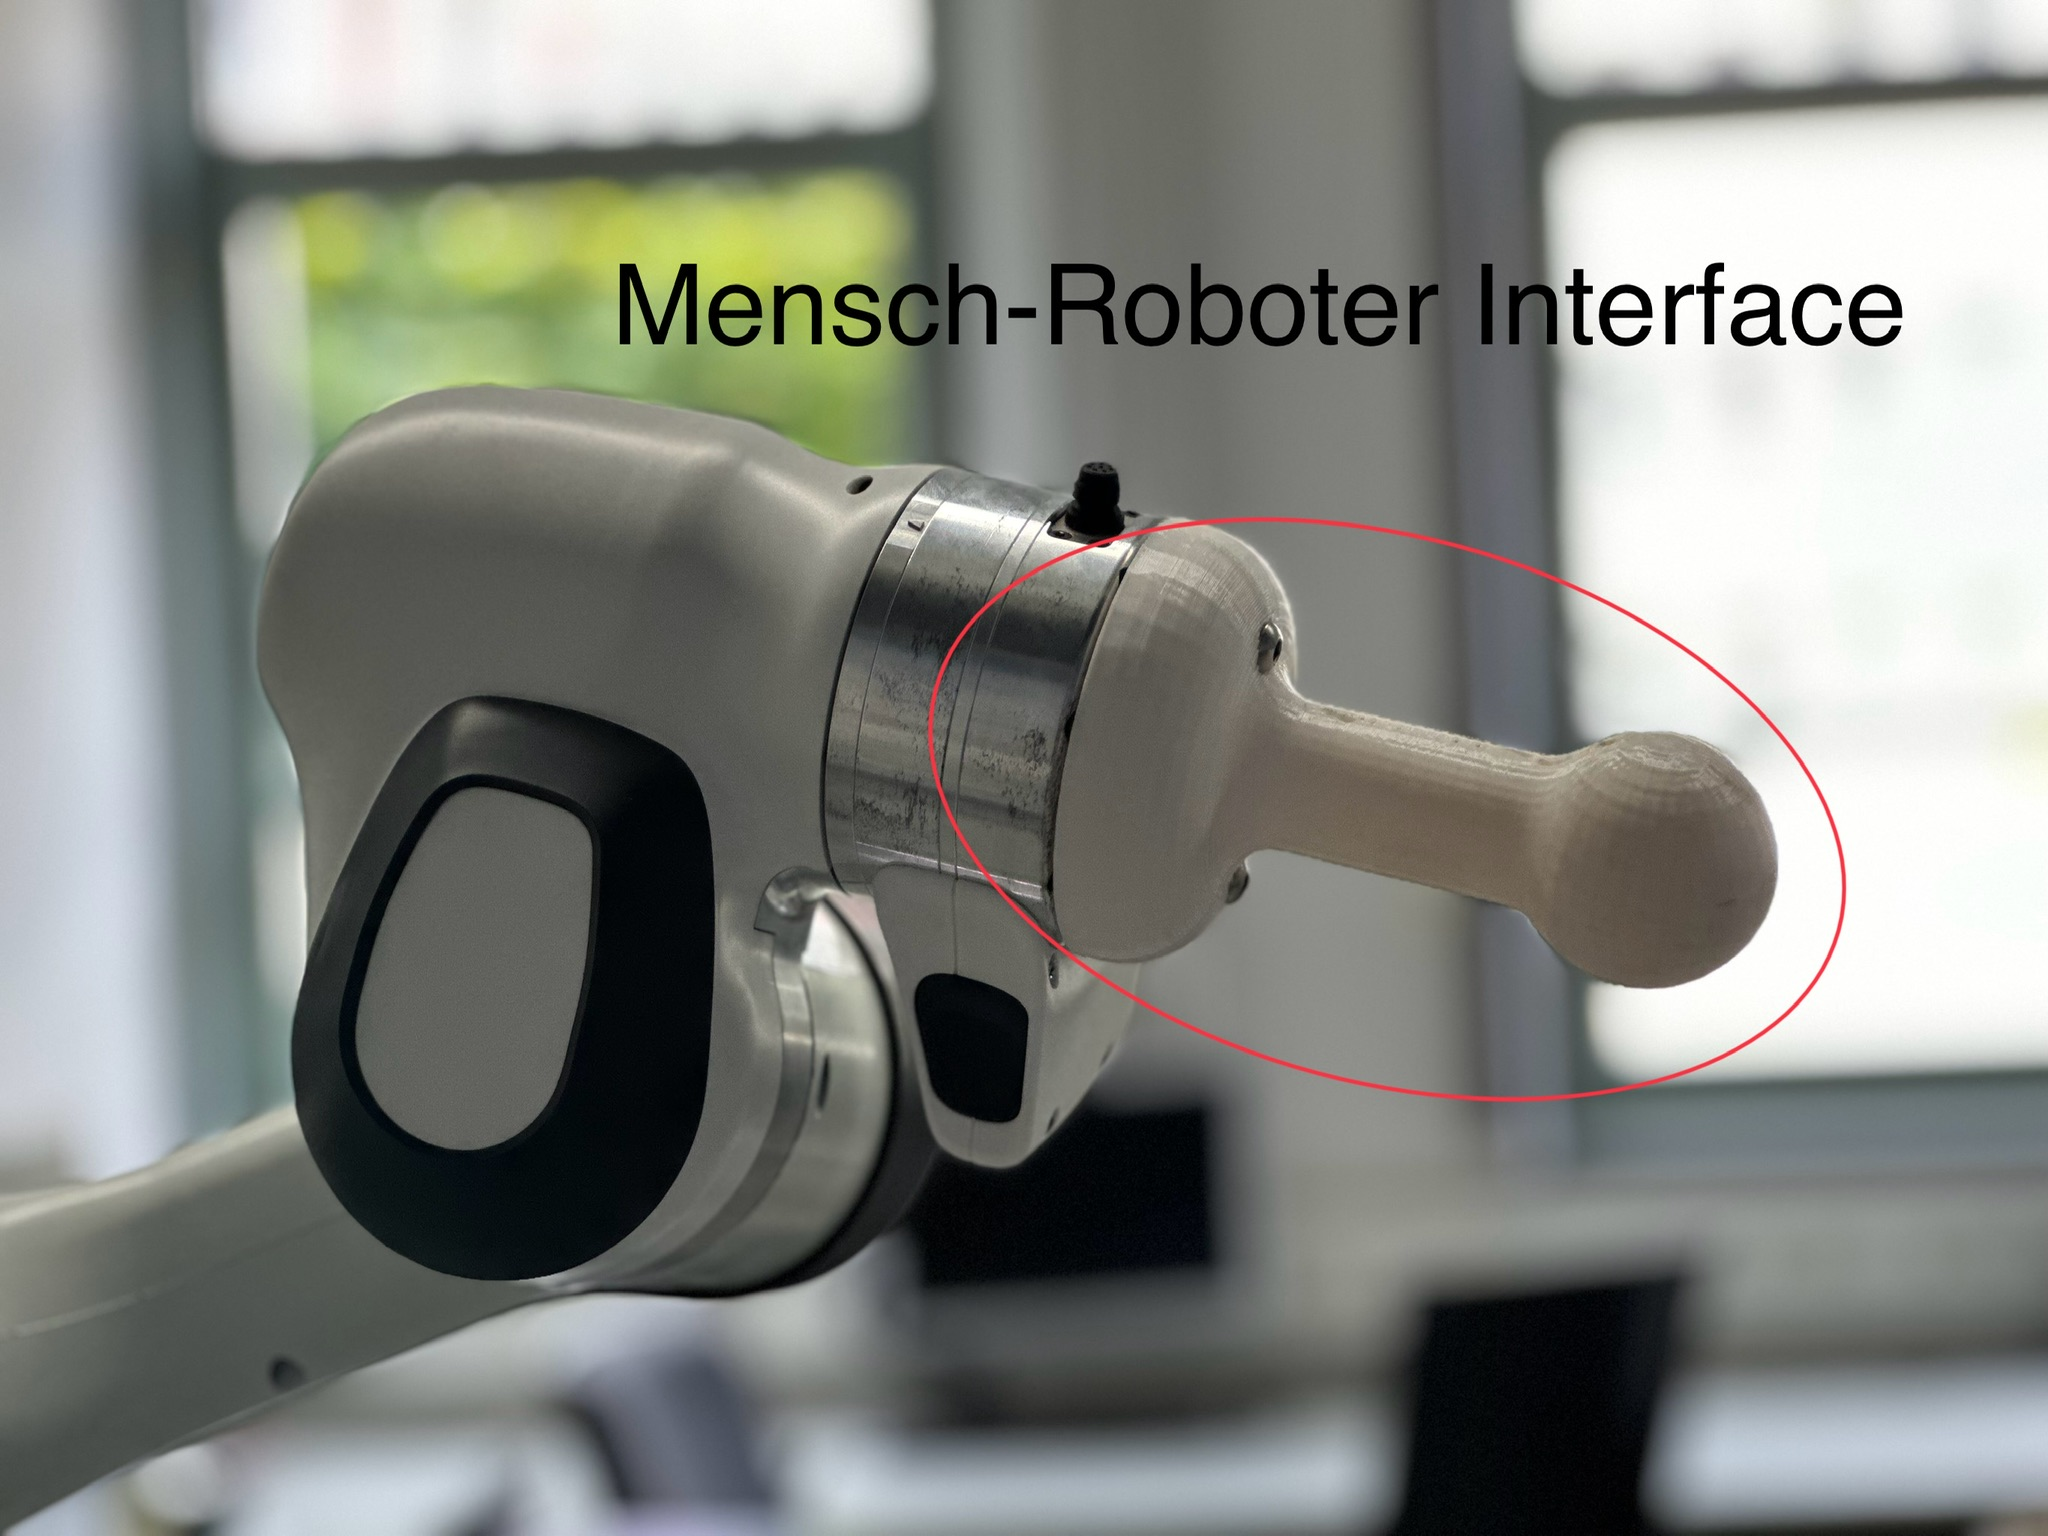
\includegraphics[width=0.45\textwidth]{pics/interface.jpeg}
    \caption{Mensch-Roboter-Schnittstelle}
    \label{fig:MRinterface}
\end{figure}

Bei der Entwicklung der Software für dieses System stand die Leistungsfähigkeit 
im Vordergrund, um eine nahtlose Benutzererfahrung zu gewährleisten. Dazu war es 
entscheidend, dass die Anwendung in Echtzeit ausgeführt werden kann, wobei eine maximale 
Zeitverzögerung von weniger als 1 Millisekunde akzeptiert wurde. Die Programmiersprache 
C++ wurde aufgrund ihrer hohen Performance ausgewählt, um diesem Anspruch gerecht zu werden. 
Die Hardware-Konfiguration bestand aus [!!!HARDWARE!!!].
Die Verarbeitung und Nutzung der 3D-Modelle wurden durch die Umwandlung der STL-Daten in 
Eigen-Matrizen optimiert. Für diesen Prozess wurde durch einen STL-Parser benutzt. Dadurch ist 
eine einfache und effiziente Handhabung der 3D-Daten innerhalb des Programms möglich.
Insgesamt zeichnet sich unsere Methodik durch die Kombination von Standardtechnologien 
und innovativen Ansätzen aus, um eine effiziente und benutzerfreundliche Lösung für haptisches 
Feedback in der Mensch-Roboter-Interaktion zu schaffen.

\section{Results}

\section{Discussion}

\section{Conclusion}

\printbibliography

\end{document}